\documentclass[11pt,a4paper]{scrartcl}
\usepackage[utf8]{inputenc}
\usepackage{textcomp}
\usepackage{lmodern}
\usepackage{amsmath}
\usepackage{amsfonts}
\usepackage{amssymb}
\usepackage{graphicx}
\usepackage[
	activate=true,
	final,
	tracking=true,
	kerning=true,
	spacing=true,
	factor=1100,
	stretch=10,
	shrink=10
]{microtype}
\usepackage{listings}
\lstset{
	frame=shadowbox,
	numbers=left,
	showstringspaces=false,
	upquote=true,
	basicstyle=\ttfamily\small,
	columns=fullflexible,
	breaklines=true,
	postbreak=\mbox{$\hookrightarrow$\space}
}

\author{Gary Moore}
\title{Network Database Applications Assignment 1: Individual Activities}

\begin{document}
	\maketitle
	
	\section{Introduction}\label{introduction}
	
	With the planning completed for the library database system, what remains to be implemented is the database itself. The database is to be implemented using Transactional Structured Query Language which will require a database server, and database management software for writing queries and executing them on the server.
	
	\section{Requirements}\label{requirements}
	
	The following software will be used:
	
	\begin{itemize}
		\item MSSQL Server 2017 for Docker
		\item SQLPro management software for macOS
	\end{itemize}
	
	I’ll be using the Docker image of SQL Server  as it can be deployed on any operating system that can run a virtual machine. It also runs from within a sandboxed container, which makes it measurably more secure than running it on the host machine. I personally needed to use a Docker image as SQL Server is not software that can run natively on macOS.
	
	Docker will likely only be used for the development of the database. When moved to a production environment, the database will likely be exported and run natively on a Windows server.
	
	Typically, SQL Management Studio by Microsoft is used to manage T-SQL databases, but due to the software only being available on one platform I used SQLPro, which has a layout that matches very closely to the Microsoft software.
	
	\section{Tables}\label{sql requirements}
	
	\subsection{tblContact}\label{tblcontact}
	
	The first table will be \texttt{tblContact} as \texttt{tblCustomer} and \texttt{tblEmployee} are dependent upon it.
	
	\lstinputlisting[language=sql]{queries/CreateTblContact.sql}
	
	The \texttt{CREATE TABLE} command will create the table \texttt{tblCustomer}, with columns then entered in the bracket delimiters. The first common is an \texttt{INT}, which is shorthand for integer. It is an auto incrementing number that is also the primary key, with \texttt{IDENTITY (1,1)} meaning it increments by one with each new field and \texttt{PRIMARY KEY} denoting that this is a fields identifying column. Each primary key is automatically enforced with constraints to ensure that a null value isn’t used, and that each field must have a unique primary key.
	
	Almost every key after the primary key uses the \texttt{VARCHAR} datatype, which can contain a string, and is of variable length. A column of this data type that’s notable is \texttt{cnPostcode}. A post code is typically considered to be fixed length, however there’s a fairly common edge case of a 6-character long post code, for example BT7 5NA. This is why \texttt{VARCHAR} is used instead of \texttt{CHAR}. Another notable aspect of these columns is most of them use the constraint \texttt{NOT NULL}, which means that a null value cannot be entered into this column.
	
	\texttt{CHAR} of length 11 is used for the phone number as an integer isn’t appropriate here because we don’t want to perform any calculations on a phone number, and it is possible to enter a value in excess of the 32bit integer limit. \texttt{CHAR} is used instead of \texttt{VARCHAR} because all UK phone numbers are of length 11.
	
	To insert fields into this table we first use the \texttt{INSERT INTO} command followed by the table name \texttt{tblContact}. Next we declare what columns we wish to input information into in delimiters separated by commas. On a new line you write the \texttt{VALUES} keyword followed by delimited entries on a new line with strings surrounded by single quotes and numbers entered without quotes separated with a comma.
	
	The command \texttt{SELECT * FROM tblContact} will display all fields in the table.
	
	\subsubsection*{Result}
	
	\begin{center}
		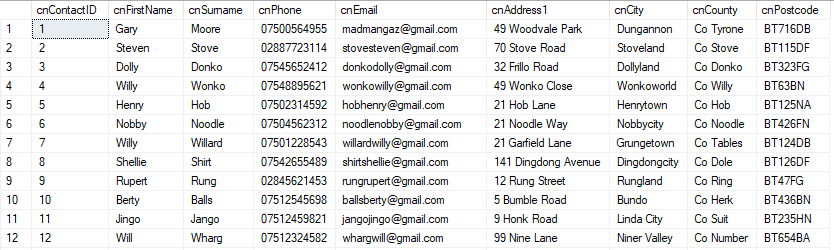
\includegraphics[width=0.95\linewidth]{images/Contact}
	\end{center}
	
	\subsection{tblCustomer}\label{tblcustomer}
	
	This is a small table as most of the details are contained in \texttt{tblContact}. The two tables use a one to many relationship avoiding redundant data.
	
	\lstinputlisting[language=sql]{queries/CreateTblCustomer.sql}
	
	This table is the first case where a foreign key is used, and a different syntax is used to create a foreign key compared to a primary key. Instead of declaring it with \texttt{PRIMARY KEY}, we write \texttt{FOREIGN KEY REFERENCES \textit{table}(\textit{column})}. The purpose of a foreign key is to link this table with another table that it references data from.
	
	We must associate each customer with its corresponding entry in tblContact, and to do this we insert the corresponding foreign key value into tblCustomer.
	
	\subsubsection*{Result}
	
	\begin{center}
		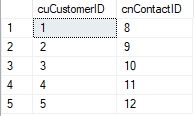
\includegraphics[width=0.3\linewidth]{images/Customer}
	\end{center}
	
	\subsection{tblEmployee}\label{tblemployee}
	
	Similarly to tblCustomer we must initialise a foreign key, however there are extra fields for this table with employee specific information.
	
	\lstinputlisting[language=sql]{queries/CreateTblEmployee.sql}
	
	Every employee will need a password to get access to the database system and appropriate permissions that will define what that employee can change in the database. For example an administrator will be able to drop and add tables, where as a user may only be able to alter or add data to the database.
	
	\subsubsection*{Result}
	
	\begin{center}
		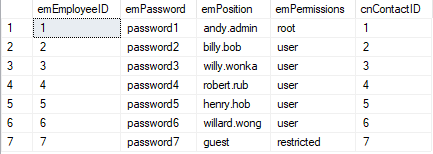
\includegraphics[width=0.7\linewidth]{images/Employee}
	\end{center}
	
	\subsection{tblAuthor}\label{tblauthor}
	
	This table will have a many to many relationship with \texttt{tblBook}. A junction table will be used between the two tables, more information will be in section \ref{tblbookauthor}.
	
	\lstinputlisting[language=sql]{queries/CreateTblAuthor.sql}
	
	For any new books that are added to the database system, the author names will go into a second document to avoid redundant data, as authors can write more than one book.
	
	\subsubsection*{Result}
	
	\begin{center}
		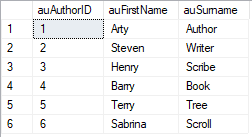
\includegraphics[width=0.4\linewidth]{images/Author}
	\end{center}
	
	\subsection{tblBook}\label{tblbook}
	
	This table has a many to many relationship with \texttt{tblAuthor}.
	
	\lstinputlisting[language=sql]{queries/CreateTblBook.sql}
	
	A unique aspect of this table; it uses the ISBN number of the book as its primary key. Because the number is so big, we use \texttt{VARCHAR} instead of the \texttt{INT} data type, which can be used as the primary key so long as it's unique. We're using a variable data type because an ISBN can be 10 or 13 digits long.
	
	We also create columns for the title and genre of the book and use \texttt{INSERT INTO} to fill out some values.
	
	\subsubsection*{Result}
	
	\begin{center}
		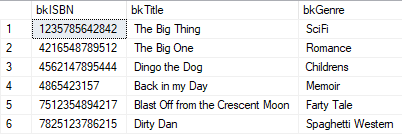
\includegraphics[width=0.65\linewidth]{images/Book}
	\end{center}
	
	\subsection{tblBookAuthor}\label{tblbookauthor}
	
	This is a junction table between \texttt{tblBook} and \texttt{tblAuthor}. The purpose of this table is to create a link between these two tables, as a many to many relationship cannot exist directly between these two tables.
	
	\lstinputlisting[language=sql]{queries/CreateTblBookAuthor.sql}
	
	This is the first instance where a composite key is created. To create one of these, we create two foreign keys from the tables \texttt{tblBook} and \texttt{tblAuthor} and then join these together using \texttt{PRIMARY KEY (auAuthorID, bkISBN)}. This joins the two together to create a unique key.
	
	\subsubsection*{Result}
	
	\begin{center}
		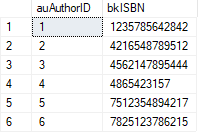
\includegraphics[width=0.35\linewidth]{images/BookAuthor}
	\end{center}
	
	\subsection{tblLeasing}\label{tblleasing}
	
	This table establishes three relationships, one with \texttt{tblCustomer}, \texttt{tblBookLeasing} and a junction table.
	
	\lstinputlisting[language=sql]{queries/CreateTblLeasing.sql}
	
	This table has some relatively complex transactions going on. To begin with, it is interacting with transactional and non-transactional tables, with transactions happening in a junction table.
	
	\subsubsection*{Result}
	
	\begin{center}
		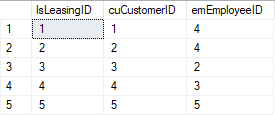
\includegraphics[width=0.45\linewidth]{images/Leasing}
	\end{center}
	
	\subsection{tblBookLeasing}\label{tblbookleasing}
	
	This is a transactional table that is a junction between \texttt{tblBook} and \texttt{tblLeasing}. It is responsible for documenting the checkout and return date 
	
	\lstinputlisting[language=sql]{queries/CreateTblBookLeasing.sql}
	
	This table makes use of a composite key, the creation of which is described in \ref{tblbookauthor}. \texttt{tblBookLeasing} is also the first use of the \texttt{DATE} data type, which is of course used for storing date information. When a customer decides to check out a book, the transaction will eventually make its way to this table, where the lease and return date are stored in \texttt{lsLeaseDate} and \texttt{lsReturnDate}.
	
	\subsubsection*{Result}
	
	\begin{center}
		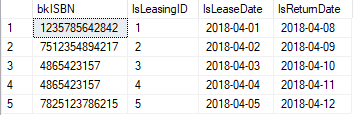
\includegraphics[width=0.65\linewidth]{images/BookLeasing}
	\end{center}
	
	\subsection{Notable Transactions}\label{notabletransactions}
	
	\subsubsection*{Adding a book}
	
	When an employee wants to add a book to the database, they will use a form that will inner join \texttt{tblAuthor}, \texttt{tblBook} and \texttt{tblBookAuthor}. This data is inserted into the table through this form.
	
	\subsubsection*{Removing a book}
	
	The process or removing a book involves some conditional logic. If the book is the only one in the system by that author, the author can be removed too. If the book has other books by the same author, the author will not be deleted. This can be done with an \texttt{IF...ELSE} statement.
		
	\subsubsection*{Leasing a book}
	
	The procedure for checking out a book uses a network of tables to carry out the transaction, again to make sure there's no data redundancy. The tables \texttt{tblCustomer}, \texttt{tblLEasing}, \texttt{tblEmployee}, \texttt{tblBook} and \texttt{tblBookLeasing} will be used to create a record of a lease with \texttt{tblContact} queried to get the customer number from any of the customers details.
	
	\section{Constraints}\label{constraints}
	
	I will make use of constraints to ensure that only valid data is entered into the database. These constraints can be created at \texttt{CREATE TABLE}, or they can be appended to the column definitions using \texttt{ALTER TABLE}.
	
	A constraint is a system in a database that applies limitations to what information can be input into a particular column in a table. An example of a constraint is \texttt{NOT NULL}, which doesn't allow the user to enter a null value into their table. Another example is \texttt{UNIQUE}, which only allows a unique value compared to other values entered into the same column to exist. Violation of a constraint will result in an error which is displayed in the SQL management software's console.
	
	I've created constraints for \texttt{tblContact}; a constraint for email, postcodes and phone numbers.
	
	\lstinputlisting[language=sql]{queries/CreateConstraints.sql}
	
	To add these constraints we need to alter the \texttt{tblContact} table and then use the \texttt{ADD} command followed by the \texttt{CONSTRAINT} keyword on a new line with the name that we'll use for the constraint. We use \texttt{CHECK} to make sure that input values abide by the defined rule in the parenthesis. A boolean value of true is generated if the value matches the pattern, allowing the database to add that value to the table.
	
	\subsection{Phone constraint}\label{phoneconstraint}
	
	Check line 3 of the example in Chapter \ref{constraints}. The requirements for the phone constraint are quite simple. Only digits can be accepted, therefore I've used the \texttt{[0-9]} wildcard to denote only digits. I've used this 11 times as the wildcard only represents a single character.
	
	\subsubsection*{Testing}
	
	In the first image I'm checking to see if the constraint works when I try to add a phone number with less than 11 digits. The constraint successfully prevents this from happening, throwing an error.
	
	\begin{center}
		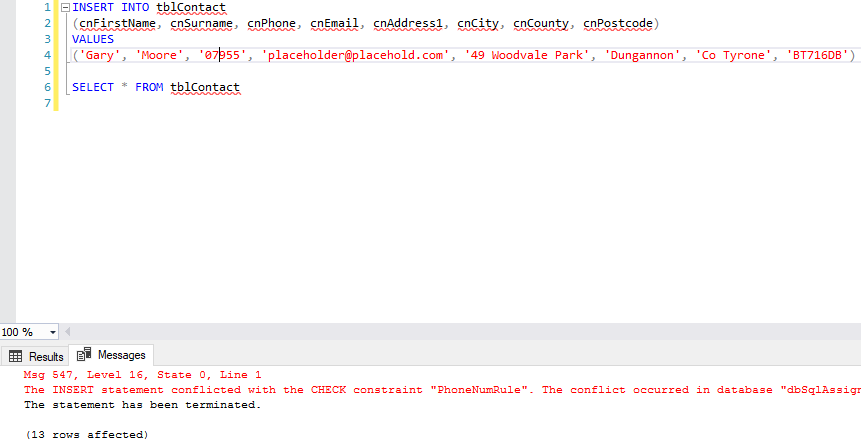
\includegraphics[width=0.9\linewidth]{images/PhoneConstraintTest1}
	\end{center}
	
	In the second image, I am trying to use letters as a phone number, however the constraint catches this, and throws out an error.
	
	\begin{center}
		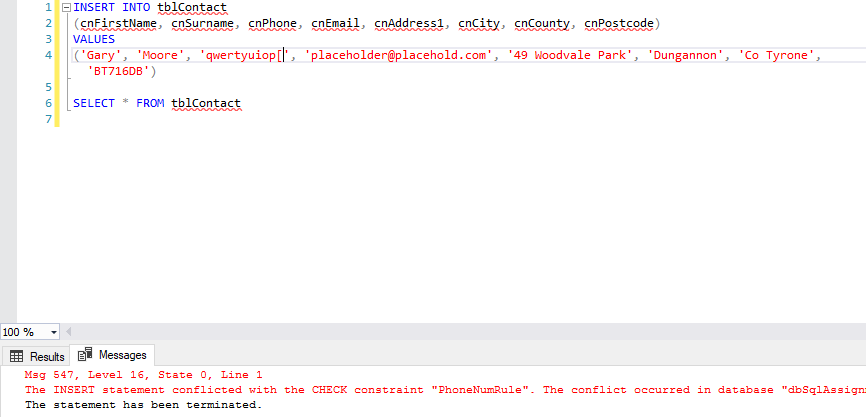
\includegraphics[width=0.9\linewidth]{images/PhoneConstraintTest2}
	\end{center}
	
	In the third image, I pass a valid phone number to test if the constraint will allow valid data to be inserted into the table. The constraint passes the test.
	
	\begin{center}
		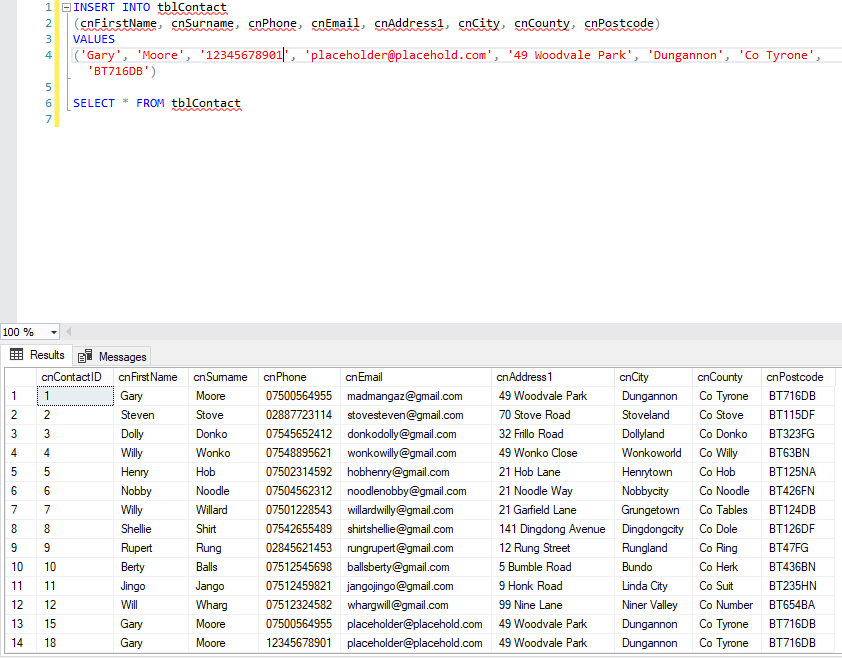
\includegraphics[width=0.9\linewidth]{images/PhoneConstraintTest3}
	\end{center}
	
	\subsection{Email constraint}\label{emailconstraint}
	
	Check line 4 of the example in Chapter \ref{constraints}. This check is slightly more complicated as i'm using the \texttt{AND} statement, which means values must pass two checks in order to be inserted into the table. First it will check if the correct email formatting is used, that is the requirement of \texttt{\&, period, username, domain name} and \texttt{tld}. I don't want an email to look like `\texttt{\&.com}', and the \texttt{\%} wildcard will allow any string with no characters up to exist there, so I have to do a second check that requires the length of the value to be greater than 6, which is the minimum for there to be information in the username and domain name. This isn't perfect however, as it could still look like this `\texttt{aa@.com}'. This constraint should however weed out the most troublesome data validation errors.
	
	Another way to do data validation that I haven't looked at is to use a Regular Expression, however this requires integrating a CLR\footnote{Common Language Runtime} function into the database solution.
	
	\subsubsection*{Testing}
	
	In the first image I am testing to see if validation works when the input is not long enough to pass. An error message is displayed and the data is not inserted into the table as it did not pass the test.
	
	\begin{center}
		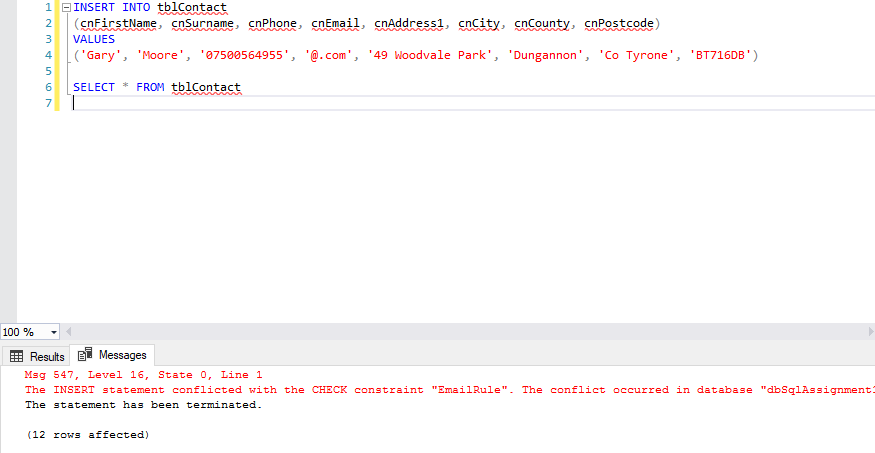
\includegraphics[width=0.9\linewidth]{images/EmailConstraintTest1}
	\end{center}
	
	In the second image I am testing to see if validation works when I only input a username without the \texttt{\@}, period, tld or domain name. The data fails the test and isn't inserted into the table.
	
	\begin{center}
		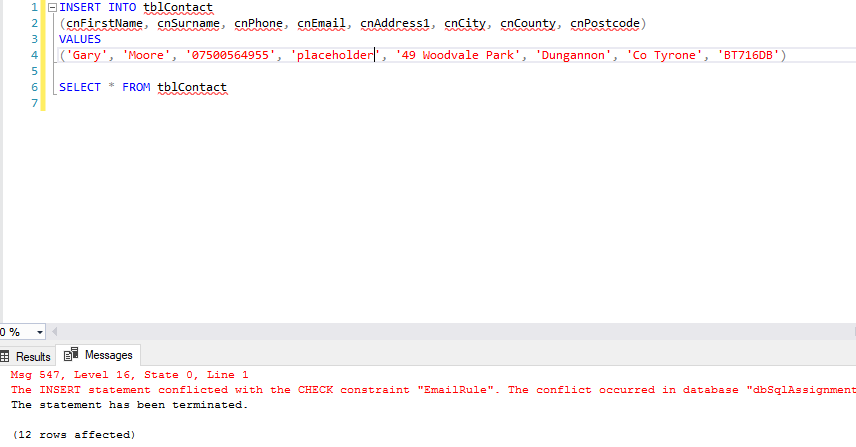
\includegraphics[width=0.9\linewidth]{images/EmailConstraintTest2}
	\end{center}
	
	In the third image, I am testing valid data to ensure that it passes the test. It does, and the data is inserted into the table.
	
	\begin{center}
		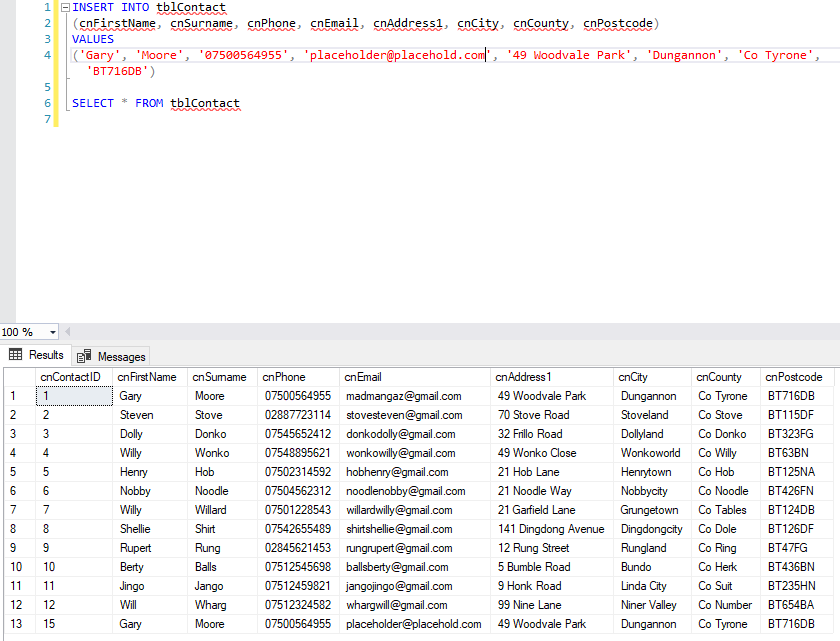
\includegraphics[width=0.9\linewidth]{images/EmailConstraintTest3}
	\end{center}
	
	\subsection{Postcode constraint}\label{postcodeconstraint}
	
	Check line 5 of the example in Chapter \ref{constraints}. A postcode can be 6 or 7 characters long, and the typical format is \texttt{[Char, Char, Num, Num, Num, Char, Char]}. The constraint needs to ensure that this formatting is used, and also that it is of length 6 or 7.
	
	In order to do this I used the wildcards \texttt{[A-Z]} and \texttt{[0-9]} where appropriate. I also used an \texttt{OR} statement that results in true if either one of the conditional statements is true.
	
	\subsubsection*{Testing}
	
	In the first image I am testing to ensure that the constraint rejects data that is too short to be a valid postcode. The constraint works as intended, and an error message is displayed with the data not being inserted into the table.
	
	\begin{center}
		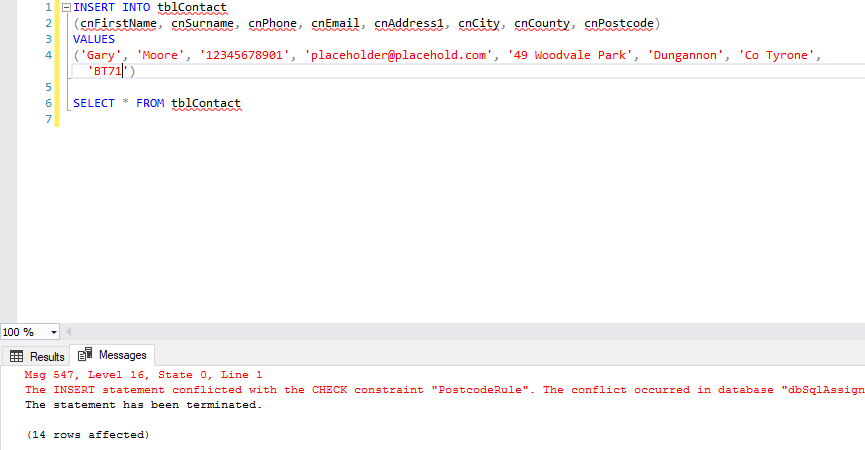
\includegraphics[width=0.9\linewidth]{images/PostcodeConstraintTest1}
	\end{center}
	
	In the second image I am testing to ensure that a 6 character postcode get successfully inserted into the table. The test shows that the validation passed, and the data goes into the table.
	
	\begin{center}
		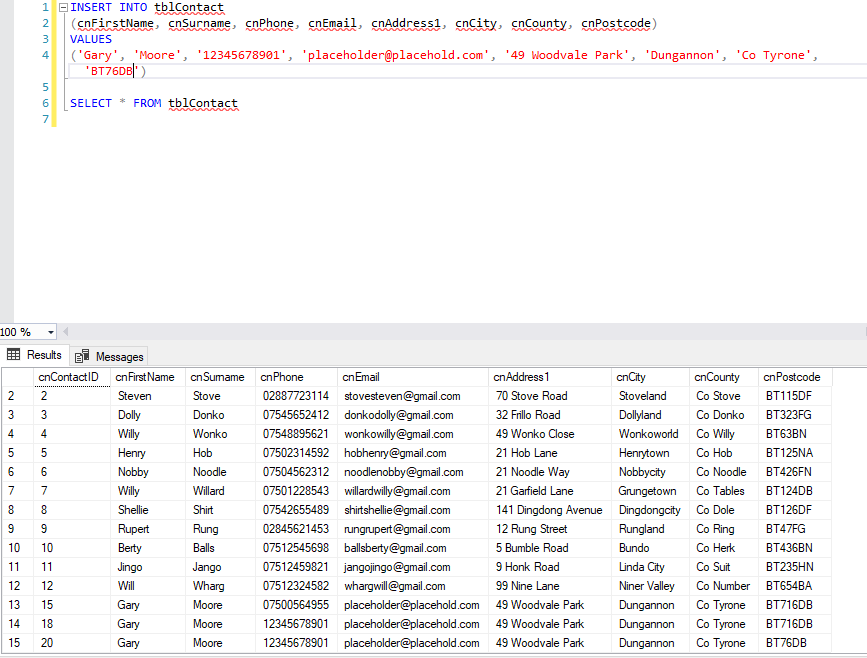
\includegraphics[width=0.9\linewidth]{images/PostcodeConstraintTest2}
	\end{center}
	
	\section{Locking}\label{locking}
	
	We use locking in databases to prevent multible users from accessing data simulatneously. The reason this is a desirable feature is because if data is accessed at the same time it can have negative side effects such as data mutation. If someone alters information in a column, and another person does the same thing, one of these transactions may get overwritten, and it would be as if one of these transactions never happened. This would be very bad in for example a bank account, where real money could be lost as a result.
\end{document}